\documentclass[border=10pt]{standalone}
\usepackage{tikz}
\usepackage{booktabs}
\usetikzlibrary{arrows.meta, positioning, calc}

\begin{document}
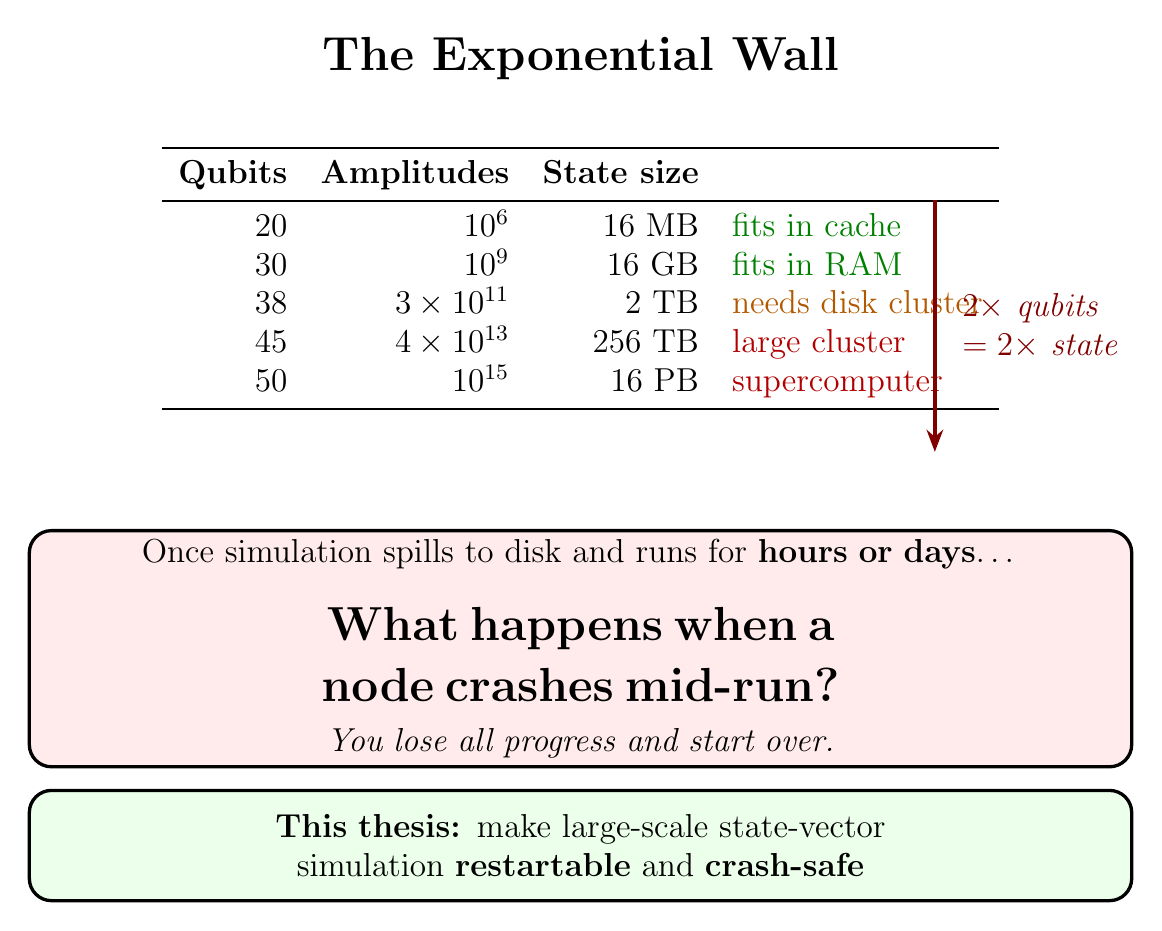
\begin{tikzpicture}[
    heading/.style={font=\LARGE\bfseries},
]

% ===================== TITLE =====================
\node[heading] at (8, 11) {The Exponential Wall};

% ===================== SCALING TABLE =====================
\node[anchor=north] at (8, 10) {
\large
\begin{tabular}{r r r l}
\toprule
\textbf{Qubits} & \textbf{Amplitudes} & \textbf{State size} & \\
\midrule
20 & $10^6$ & 16 MB & \textcolor{green!50!black}{fits in cache} \\
30 & $10^9$ & 16 GB & \textcolor{green!50!black}{fits in RAM} \\
38 & $3 \times 10^{11}$ & 2 TB & \textcolor{orange!70!black}{needs disk cluster} \\
45 & $4 \times 10^{13}$ & 256 TB & \textcolor{red!70!black}{large cluster} \\
50 & $10^{15}$ & 16 PB & \textcolor{red!70!black}{supercomputer} \\
\bottomrule
\end{tabular}
};

% ===================== ARROW showing exponential growth =====================
\draw[very thick, red!50!black, -{Stealth[length=8pt]}]
    (12.5, 9.2) -- (12.5, 6.0)
    node[midway, right=6pt, font=\large\itshape, text=red!50!black, align=left]
    {$2\times$ qubits\\$= 2\times$ state};

% ===================== THE QUESTION =====================
\node[draw, very thick, fill=red!8, rounded corners=8pt,
      minimum width=14cm, minimum height=2.5cm,
      text width=13cm, align=center,
      font=\large] at (8, 3.5) {
    Once simulation spills to disk and runs for \textbf{hours or days}\ldots\\[6pt]
    \LARGE\bfseries
    What happens when a node crashes mid-run?\\[4pt]
    \large\normalfont\itshape
    You lose all progress and start over.
};

% ===================== THIS THESIS =====================
\node[draw, very thick, fill=green!8, rounded corners=8pt,
      minimum width=14cm, minimum height=1.4cm,
      text width=13cm, align=center,
      font=\large] at (8, 1) {
    \textbf{This thesis:} make large-scale state-vector simulation
    \textbf{restartable} and \textbf{crash-safe}
};

\end{tikzpicture}
\end{document}
